\chapter{Thực nghiệm, kết quả và thảo luận}
\section{Thiết lập thực nghiệm}
Thực nghiệm sử dụng CSV gốc của UCI đã xác thực dấu băm, phép chia stratified seed 42 và ba pipeline mô hình trong Chương 5. Train có 6.400 bản ghi, trong đó 217 hỏng; validation có 1.600 bản ghi, trong đó 54 hỏng; test có 2.000 bản ghi, trong đó 68 hỏng. Tỷ lệ dương gần như bằng nhau giữa ba tập. Tất cả số liệu so sánh mô hình được tính trên validation; chỉ mô hình và ngưỡng đã chọn được đánh giá trên test. Máy tính sử dụng Python 3.13.12 với các phiên bản thư viện ghi ở Chương 6.

Quy trình chạy là: tải dữ liệu, huấn luyện ba ứng viên, xuất bundle và metric, tạo hai lô giám sát, chạy monitor, rồi sinh bằng chứng báo cáo. Mọi hình trong chương này được tạo từ CSV hoặc hiện vật của chính quy trình đó. Số liệu làm tròn ba chữ số thập phân để trình bày; tệp JSON giữ giá trị đầy đủ. Do chỉ có một phép chia, kết quả không bao gồm độ lệch chuẩn trên nhiều seed hay khoảng tin cậy. Đây là một hạn chế khi diễn giải khác biệt nhỏ giữa các thuật toán.

\section{So sánh ba ứng viên trên validation}
\begin{table}[H]\centering\caption{So sánh mô hình trên tập validation; precision, recall và $F_2$ tại ngưỡng riêng của từng mô hình}\label{tab:validation}
\begin{tabular}{lrrrr}\toprule Mô hình & AP & Precision & Recall & $F_2$\\\midrule
Logistic Regression & 0,420 & 0,285 & 0,685 & 0,535 \\
Random Forest & 0,712 & 0,440 & 0,815 & 0,696 \\
XGBoost & 0,780 & 0,581 & 0,796 & 0,741 \\
\bottomrule

\end{tabular}\end{table}
Logistic Regression đạt AP 0,420; Random Forest đạt 0,712; XGBoost đạt 0,780. Chênh lệch giữa đường chuẩn tuyến tính và hai mô hình cây cho thấy các quan hệ phi tuyến hoặc tương tác có thể quan trọng trong dataset này. Không thể từ đó kết luận một thuật toán luôn tốt hơn trên dữ liệu công nghiệp khác. Trong cùng phép chia, XGBoost đứng đầu theo quy tắc AP đã định trước, nên được chọn. Precision 0,581 và recall 0,796 của XGBoost trên validation là tại ngưỡng 0,15; Random Forest dùng 0,21 và Logistic Regression dùng 0,74.

\begin{figure}[H]\centering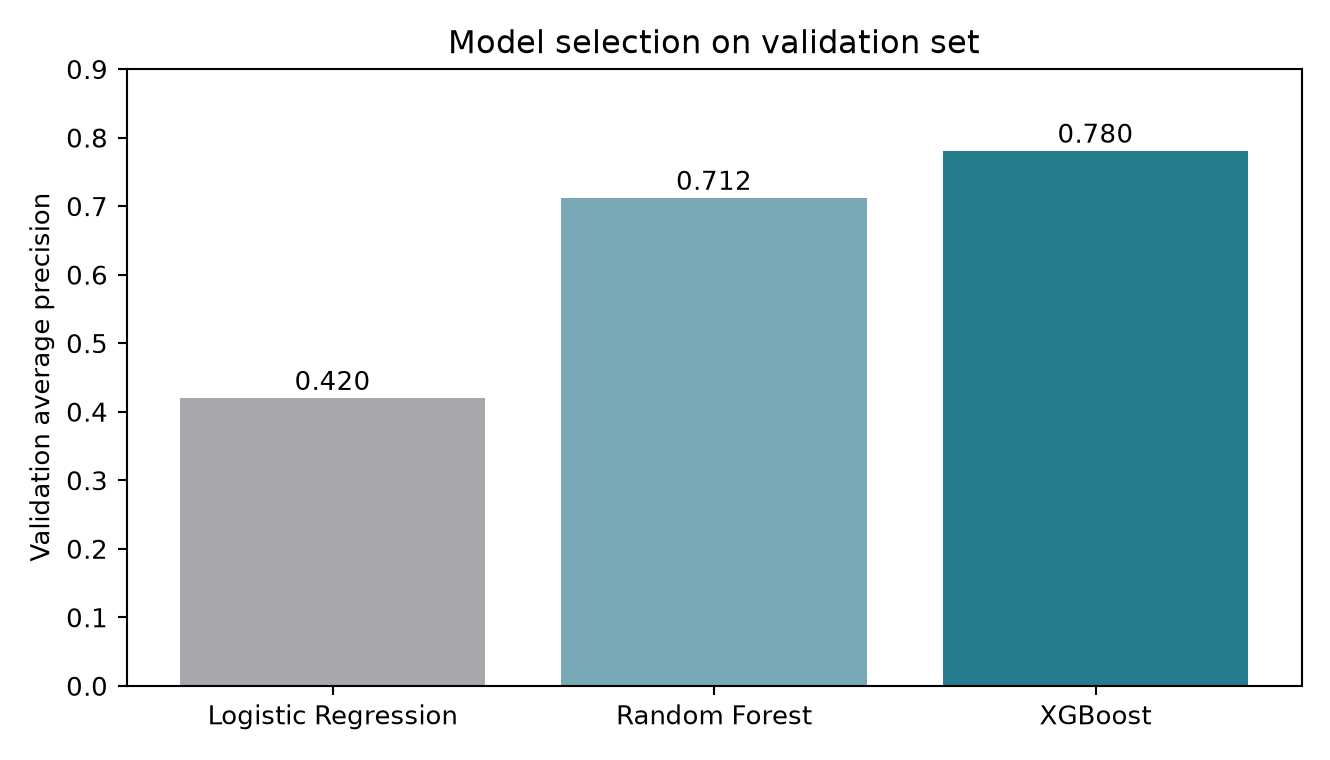
\includegraphics[width=.86\textwidth]{validation_comparison.png}\caption{Average precision của ba ứng viên trên validation.}\label{fig:validation}\end{figure}

AP là chỉ số xếp hạng tổng hợp, không nói trực tiếp số ca bỏ sót tại ngưỡng dùng trong dịch vụ. Vì vậy, bên cạnh AP, nhóm chọn ngưỡng bằng $F_2$ trên validation. Hình~\ref{fig:threshold} biểu diễn điểm $F_2$ của XGBoost theo dải 91 ngưỡng đã quét. Việc chỉ tối ưu trong một dải và bước 0,01 có nghĩa 0,15 là tối ưu \emph{trên lưới thử này}, không phải nghiệm liên tục tối ưu tuyệt đối. Nếu thay đổi mục tiêu ưu tiên hoặc chi phí cảnh báo sai, ngưỡng có thể thay đổi đáng kể.

\begin{figure}[H]\centering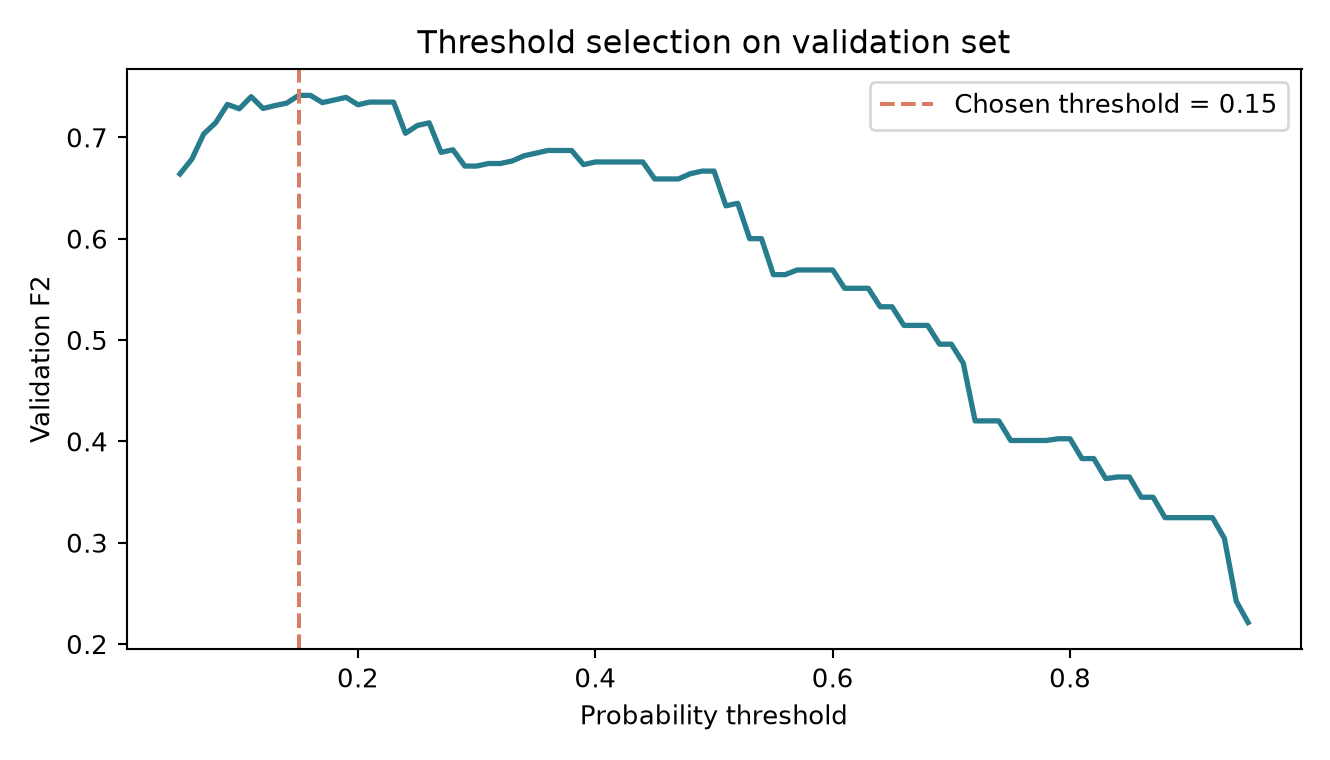
\includegraphics[width=.9\textwidth]{threshold_f2.png}\caption{Điểm $F_2$ trên validation theo ngưỡng của XGBoost; dấu đánh dấu chỉ ngưỡng được lưu.}\label{fig:threshold}\end{figure}

\section{Kết quả test của mô hình được chọn}
XGBoost với ngưỡng 0,15 đạt AP 0,825, ROC-AUC 0,974, precision 0,614, recall 0,794, $F_1$ 0,692 và $F_2$ 0,750 trên test. Cần phân biệt AP 0,825 với precision 0,614: AP đánh giá toàn dải ngưỡng, còn precision chỉ đánh giá các cảnh báo khi $p\geq0,15$. Chỉ số ROC-AUC cao cho thấy khả năng xếp thứ tự hai lớp trên tập test này, nhưng không trực tiếp phản ánh số cảnh báo sai trong lịch làm việc của nhân viên bảo trì.

\begin{table}[H]\centering\caption{Ma trận nhầm lẫn trên test, ngưỡng 0,15}\label{tab:confusion}
\begin{tabular}{lrr}\toprule Thực tế / dự đoán & Không hỏng & Hỏng\\\midrule
Không hỏng & 1.898 (TN) & 34 (FP)\\
Hỏng & 14 (FN) & 54 (TP)\\\bottomrule
\end{tabular}\end{table}
Trong 68 bản ghi hỏng, hệ thống phát hiện đúng 54 và bỏ sót 14. Trong 1.932 bản ghi không hỏng, 34 nhận cảnh báo sai. Tổng số cảnh báo là $54+34=88$, nên precision bằng $54/88\approx0,614$. Recall bằng $54/68\approx0,794$. Các phép tính này kiểm tra độc lập tính nhất quán của metric lưu trong JSON. Về vận hành, 34 cảnh báo sai có thể tạo thêm công việc kiểm tra; 14 ca bỏ sót vẫn là rủi ro. Không có dữ liệu chi phí, nên báo cáo không định giá tiền cho hai loại sai lầm.

\begin{figure}[H]\centering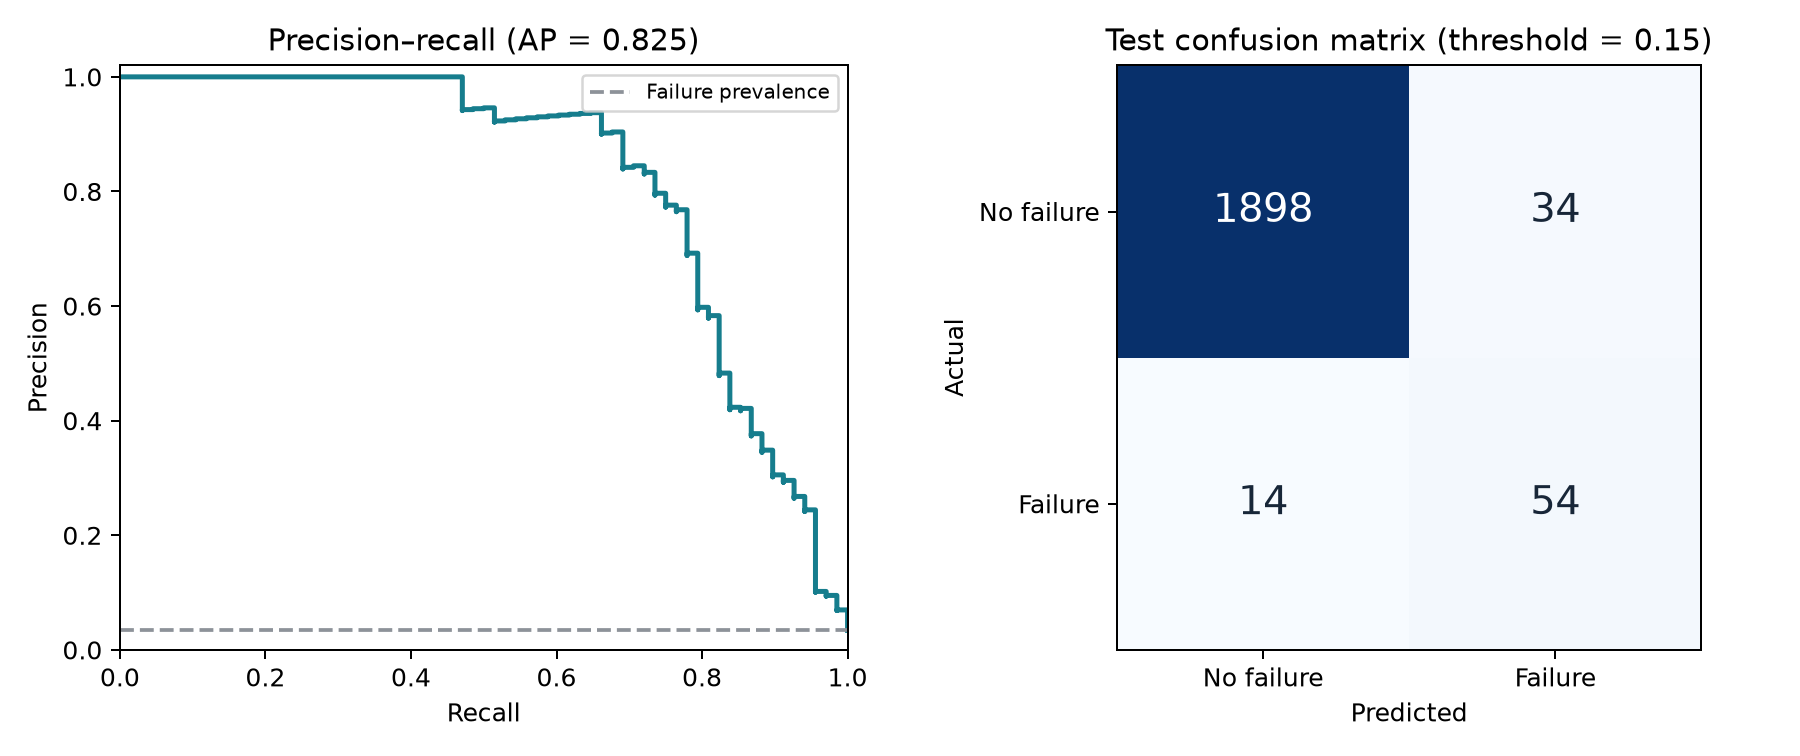
\includegraphics[width=.96\textwidth]{model_evaluation.png}\caption{Đường precision--recall và ma trận nhầm lẫn test của mô hình được chọn.}\label{fig:model_eval}\end{figure}

Độ chính xác tổng thể tính từ ma trận là $(1898+54)/2000=97,6\%$, nhưng con số này ít giúp đánh giá lớp hỏng khi tỷ lệ dương chỉ 3,39\%. Mốc luôn dự đoán không hỏng trên toàn bộ dữ liệu đã đạt accuracy 96,61\%. Chênh lệch giữa hai accuracy nhìn có vẻ nhỏ dù mô hình thật phát hiện 54 ca hỏng; đây là lý do báo cáo không dùng accuracy để chọn mô hình. Độ bao phủ của cảnh báo, precision và số FP/FN trực tiếp hơn cho quyết định kiểm tra.

\section{Diễn giải thuộc tính}
Hình~\ref{fig:importance} hiển thị mức độ quan trọng thuộc tính của XGBoost trong bundle đã huấn luyện. Đây là thống kê phụ thuộc cách xây dựng cây và cách thư viện tổng hợp đóng góp của các lần tách. Nó hữu ích để kiểm tra sơ bộ xem mô hình có dựa vào các biến cảm biến hợp lệ, nhưng không chứng minh rằng thay đổi một cảm biến sẽ gây ra hoặc ngăn hỏng máy. Các biến có tương quan có thể chia sẻ hoặc thay đổi thứ hạng độ quan trọng khi dữ liệu và seed thay đổi. Để giải thích từng cảnh báo với người vận hành, cần phương pháp diễn giải cục bộ và kiểm chứng với chuyên gia, chưa có trong bản mẫu.

\begin{figure}[H]\centering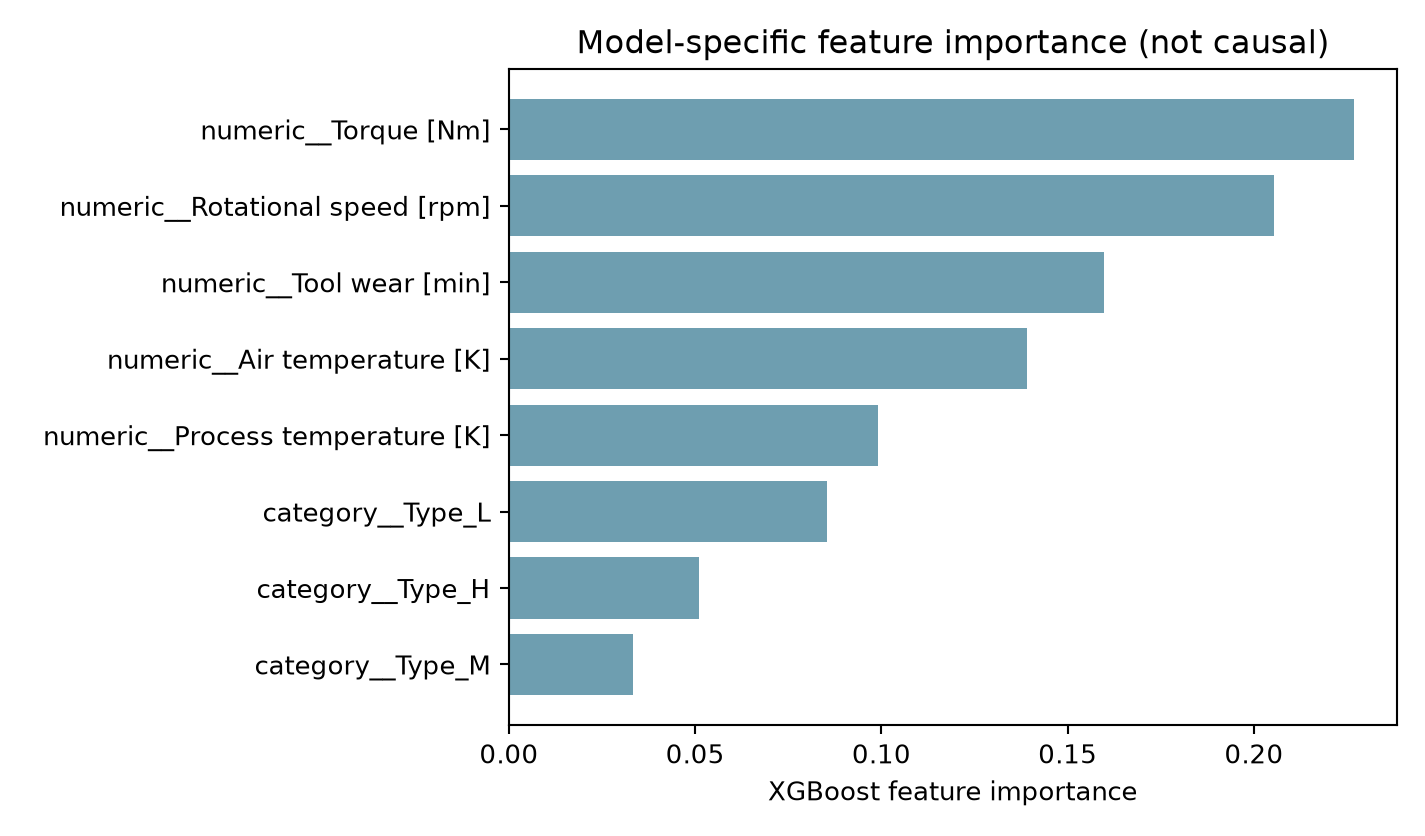
\includegraphics[width=.9\textwidth]{feature_importance.png}\caption{Độ quan trọng thuộc tính của XGBoost; chỉ diễn giải theo mô hình đã khớp.}\label{fig:importance}\end{figure}

\section{Phân tích lỗi sau đánh giá}
Sau khi cố định mô hình và ngưỡng, nhóm khảo sát các lỗi trên test để hiểu ý nghĩa của ma trận nhầm lẫn. Phân tích này chỉ mang tính mô tả hậu nghiệm: nó không được dùng để chọn lại thuật toán hoặc ngưỡng. Bảng~\ref{tab:subgroup} tách số dự đoán theo \src{Type}. Loại L có 38 bản ghi hỏng, phát hiện đúng 29 và bỏ sót 9; loại M có 25 bản ghi hỏng, phát hiện đúng 21 và bỏ sót 4; loại H có 5 bản ghi hỏng, phát hiện đúng 4 và bỏ sót 1. Các số dương của nhóm H rất ít, nên một trường hợp thêm hoặc bớt sẽ làm tỷ lệ thay đổi mạnh. Báo cáo vì vậy đưa số đếm thay vì khẳng định mô hình công bằng hoặc ổn định theo nhóm.

\begin{table}[H]\centering\caption{Kết quả test theo loại sản phẩm, chỉ để phân tích hậu nghiệm}\label{tab:subgroup}
\begin{tabular}{lrrrrr}\toprule Loại & Số dòng & Số hỏng & TP & FN & FP\\\midrule
L & 1.170 & 38 & 29 & 9 & 20 \\
M & 616 & 25 & 21 & 4 & 11 \\
H & 214 & 5 & 4 & 1 & 3 \\
\bottomrule

\end{tabular}\end{table}

Tổng TP, FN và FP theo ba nhóm phải lần lượt bằng 54, 14 và 34 như Bảng~\ref{tab:confusion}. Việc tự động kiểm tra tổng từ dự đoán của bundle trước khi sinh bảng giúp tránh lỗi sao chép thủ công. Không nên dùng bảng này để suy luận nguyên nhân khác biệt giữa các loại sản phẩm: mỗi nhóm có thể có phân phối tốc độ, mô-men hoặc hao mòn khác nhau, trong khi tập test không đủ lớn để đánh giá có điều chỉnh theo các biến đó.

\begin{table}[H]\centering\caption{Trung bình một số biến của bốn loại kết quả trên test}\label{tab:error-profiles}
\begin{tabular}{lrrrr}\toprule Nhóm & Số dòng & Xác suất & Torque (Nm) & Tool wear (min)\\\midrule
TP & 54 & 0,728 & 52,62 & 145,46 \\
FN & 14 & 0,051 & 40,65 & 183,64 \\
FP & 34 & 0,331 & 47,95 & 158,79 \\
TN & 1.898 & 0,006 & 39,41 & 106,54 \\
\bottomrule

\end{tabular}\end{table}

Bảng~\ref{tab:error-profiles} so sánh trung bình xác suất mà mô hình gán và hai biến vật lý theo bốn ô ma trận. Trong 14 âm giả, xác suất trung bình khoảng 0,051, thấp hơn ngưỡng 0,15; mức hao mòn trung bình của nhóm này khoảng 183,64 phút, cao hơn nhóm dương thật. Điều đó nhắc rằng một biến riêng lẻ cao không đủ để mô hình phát cảnh báo, vì dự đoán còn phụ thuộc các thuộc tính và tương tác khác. Trong 34 dương giả, xác suất trung bình khoảng 0,331; mô-men xoắn trung bình 47,95 Nm. Các trung bình này là mô tả của các tập con nhỏ, không phải quy tắc chẩn đoán hoặc giải thích nhân quả cho từng trường hợp.

Một bước phân tích tiếp theo nên mở từng bản ghi FN với thông tin thiết bị và thời điểm, hỏi chuyên gia liệu nhãn có chính xác, cảm biến có hoạt động bình thường và hành động kiểm tra nào đã xảy ra. Dữ liệu AI4I không cung cấp chuỗi bối cảnh đó. Việc chỉ dựa vào một biểu đồ độ quan trọng toàn cục để giải thích một âm giả cụ thể sẽ dễ dẫn đến kết luận quá mức. Nhóm giữ bảng lỗi ở mức thống kê và ghi rõ giới hạn này.

\section{Thử nghiệm giám sát dữ liệu đầu vào}
Tham chiếu của monitor là 6.400 bản ghi train. Hai lô thử nghiệm cùng có 500 bản ghi được lấy từ phần dữ liệu giữ lại. Lô bình thường giữ nguyên các phép đo; lô dịch chuyển được tạo có chủ đích bằng cộng 5 K vào nhiệt độ không khí, cộng 10 Nm vào mô-men xoắn và đặt 60\% bản ghi thành loại H. Như vậy thí nghiệm kiểm tra khả năng phát hiện của monitor trước một thay đổi đã biết, không mô phỏng một chuyển dịch tự nhiên trong nhà máy. Dữ liệu thử giám sát không được dùng để chọn mô hình hay hiệu chỉnh ngưỡng test.

\begin{table}[H]\centering\caption{Thống kê drift của hai lô; Type dùng total variation, biến số dùng KS}\label{tab:drift}
\begin{tabular}{lrrrr}\toprule Thuộc tính & Bình thường & Dịch chuyển & Ngưỡng & Cảnh báo\\\midrule
Type & 0,009 & 0,541 & 0,10 & Có \\
Air temperature & 0,033 & 0,756 & 0,20 & Có \\
Process temperature & 0,038 & 0,038 & 0,20 & Không \\
Rotational speed & 0,040 & 0,040 & 0,20 & Không \\
Torque & 0,042 & 0,399 & 0,20 & Có \\
Tool wear & 0,057 & 0,057 & 0,20 & Không \\
\bottomrule

\end{tabular}\end{table}
Lô bình thường có trạng thái \src{ok}; sáu thống kê đều dưới ngưỡng. Lô dịch chuyển có trạng thái \src{alert}, và ba biến được nêu tên là \src{Type}, \src{Air temperature [K]} và \src{Torque [Nm]}. Khoảng cách TV của Type tăng từ 0,009 lên 0,541; thống kê KS của nhiệt độ không khí từ 0,033 lên 0,756; mô-men xoắn từ 0,042 lên 0,399. Các biến còn lại giữ thống kê gần như không đổi. Với biến số, điều kiện cảnh báo còn yêu cầu p-value $<0,01$, không chỉ vượt ngưỡng KS; bảng rút gọn không hiển thị p-value nhưng báo cáo JSON lưu đầy đủ.

\begin{figure}[H]\centering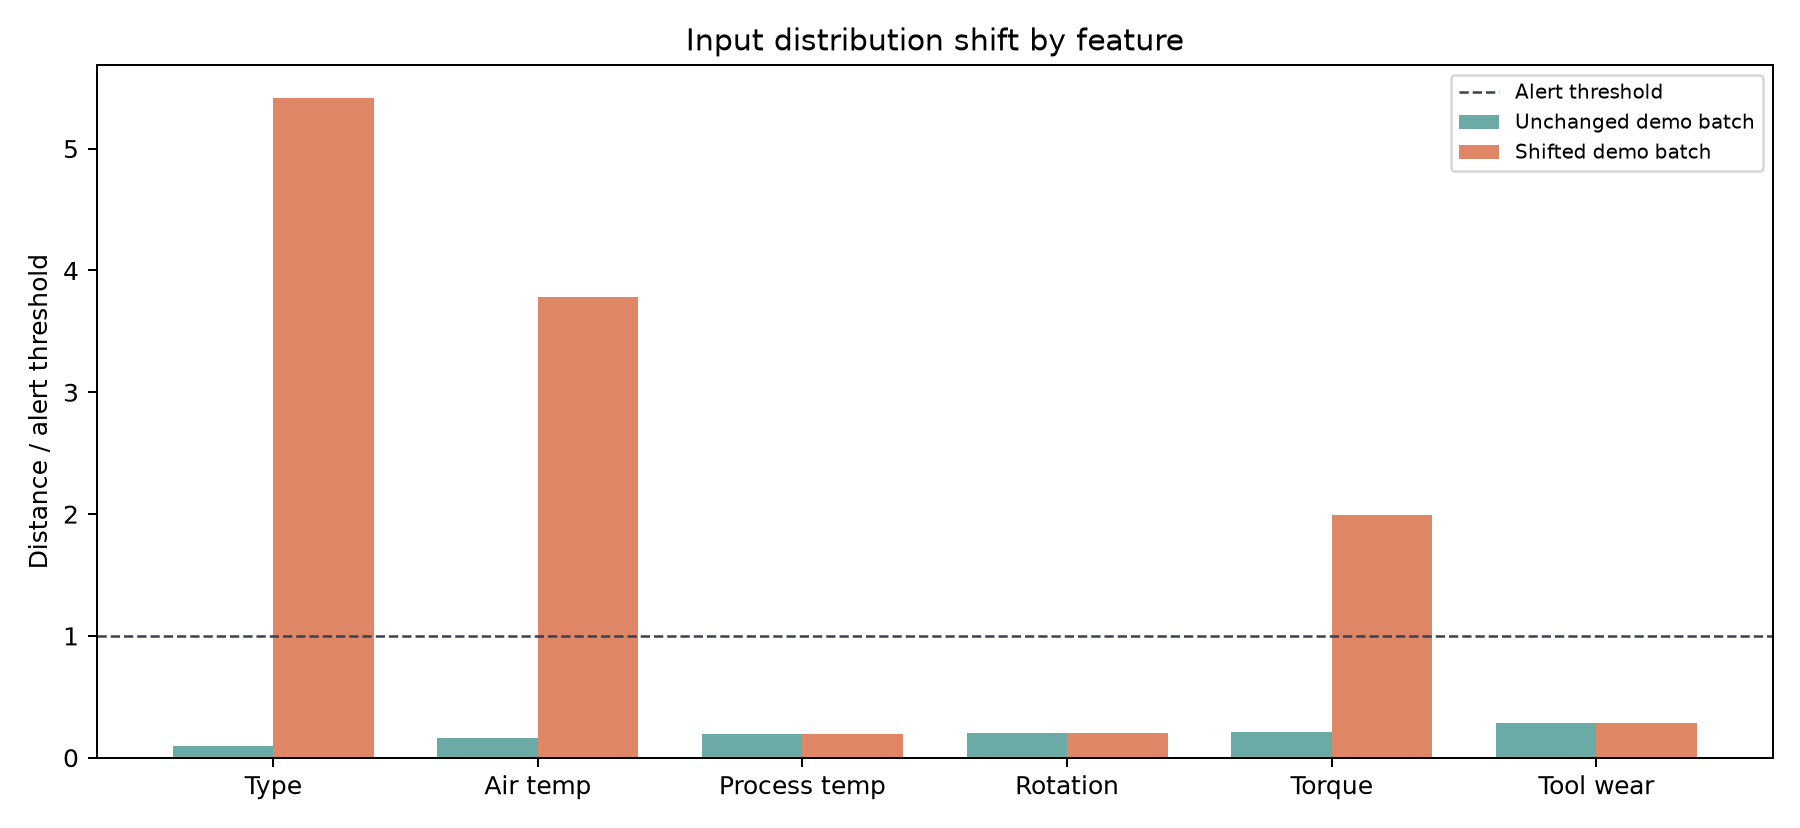
\includegraphics[width=.98\textwidth]{drift_scores.png}\caption{Thống kê so sánh từng thuộc tính giữa lô bình thường, lô dịch chuyển và tập train.}\label{fig:drift}\end{figure}

Một hệ thống phát hiện đúng ba biến được sửa là kiểm tra logic hữu ích. Nó không chứng minh ngưỡng hiện tại có tỷ lệ báo giả phù hợp trong dữ liệu thật. Lô bình thường là mẫu từ cùng nguồn, nên tương đối dễ đạt \src{ok}. Ngoài ra, monitor chỉ đo phân phối từng thuộc tính riêng lẻ; quan hệ giữa hai cảm biến có thể thay đổi mà các phân phối biên vẫn gần như cũ. Khi triển khai thật, cần theo dõi thêm tỷ lệ giá trị thiếu, miền hợp lệ theo thiết bị, tần suất dự đoán, nhãn đến trễ và chỉ số mô hình sau khi có nhãn.

\section{Kiểm tra khả năng tái tạo và vận hành}
Quy trình \src{dvc repro} làm rõ rằng dữ liệu, mã và cấu hình nào dẫn tới hiện vật. \src{dvc.lock} ghi trạng thái các giai đoạn; \src{metrics.json} ghi kết quả số; MLflow ghi lịch sử run; nguồn LaTeX trỏ vào những hiện vật này khi dựng bảng và hình. Khi API chạy, \src{/health} kiểm tra mô hình nạp được, còn \src{/predict} thực hiện một suy luận theo schema. Các thành phần này đã được thiết kế để kiểm tra những rủi ro khác nhau: DVC về phụ thuộc pipeline, MLflow về dấu vết thử nghiệm, API về hợp đồng phục vụ, monitor về dữ liệu đầu vào.

Tính tái tạo ở đây vẫn có điều kiện. Bước download cần UCI còn truy cập được; một số gói trong \src{pyproject.toml} có khoảng phiên bản; phần cứng và hệ điều hành khác có thể tạo sai khác số thực nhỏ. Tệp dữ liệu gốc có hash cụ thể nên sai khác nội dung sẽ được phát hiện. Với yêu cầu lặp lại chặt chẽ hơn, nhóm sẽ cố định lockfile môi trường, lưu dữ liệu và mô hình trong remote có phiên bản, đồng thời ghi commit Git vào mỗi MLflow run.

\section{Những gì kết quả chưa chứng minh}
AP và recall trên test phản ánh một phép chia ngẫu nhiên của dữ liệu tổng hợp. Chúng chưa đo khả năng khái quát sang nhà máy khác, dòng máy khác hoặc năm vận hành khác. Nhãn tại một bản ghi hiện tại cũng không cung cấp chân trời dự báo, vì vậy chưa thể tính ``phát hiện trước bao lâu''. Với một ứng dụng bảo trì thật, việc cảnh báo sau khi máy đã hỏng có thể không đáp ứng nhu cầu. Cần thu thập chuỗi thời gian trước sự cố, xác định mốc cảnh báo, loại bỏ mọi thông tin chỉ xuất hiện sau sự cố và kiểm tra theo thiết bị/thời gian.

Thử nghiệm drift chỉ minh họa phát hiện biến đổi đầu vào được cố ý chèn. Nó không xác nhận hiệu năng mô hình giảm khi có drift; có loại drift không ảnh hưởng đến nhãn, và cũng có sự thay đổi quan hệ $P(Y\mid X)$ mà các phân phối biên đầu vào không báo rõ. Không nên tự động huấn luyện lại chỉ vì một thống kê vượt ngưỡng. Hệ thống vận hành cần quy trình xem xét cảnh báo, lấy mẫu nhãn, so sánh mô hình mới với mô hình đang dùng và khả năng quay lại phiên bản trước.

